\documentclass[border=5pt]{standalone}
\usepackage{pgfplots}
\pgfplotsset{compat=1.18}
\usepackage{siunitx}
\usepackage{tikz}
\usetikzlibrary{calc}

\definecolor{barblue}{RGB}{31,119,180}

\begin{document}

% First bar chart - Average training time per epoch
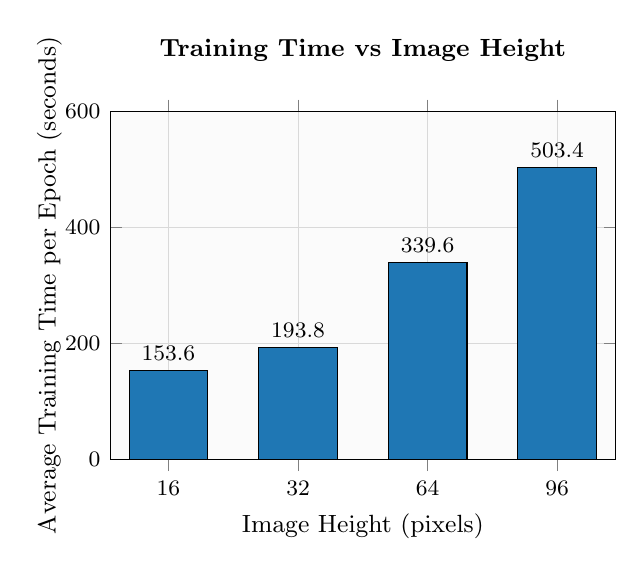
\begin{tikzpicture}
    \begin{axis}[
        width=8cm,
        height=6cm,
        ybar,
        bar width=1cm,
        xlabel={Image Height (pixels)},
        ylabel={Average Training Time per Epoch (seconds)},
        ylabel style={yshift=-0.2cm},
        symbolic x coords={16,32,64,96},
        xtick=data,
        ymin=0,
        ymax=600,
        nodes near coords,
        nodes near coords align={vertical},
        every node near coord/.style={font=\footnotesize},
        grid=both,
        grid style={line width=.1pt, draw=gray!10},
        major grid style={line width=.2pt,draw=gray!30},
        title={Training Time vs Image Height},
        axis background/.style={fill=gray!3},
        title style={yshift=3mm, font=\small\bfseries},
        label style={font=\small},
        tick label style={font=\footnotesize},
        enlarge x limits=0.15
    ]
    
    % Data extracted from your logs (converted from mm:ss to seconds)
    \addplot[fill=barblue] coordinates {
        (16, 153.6) % Average of 2:33.6 (153.6s)
        (32, 193.8) % Average of 3:13.8 (193.8s)
        (64, 339.6) % Average of 5:39.6 (339.6s)
        (96, 503.4) % Average of 8:23.4 (503.4s)
    };
    
    \end{axis}
\end{tikzpicture}

\hspace{1cm}

% Second bar chart - Number of model parameters
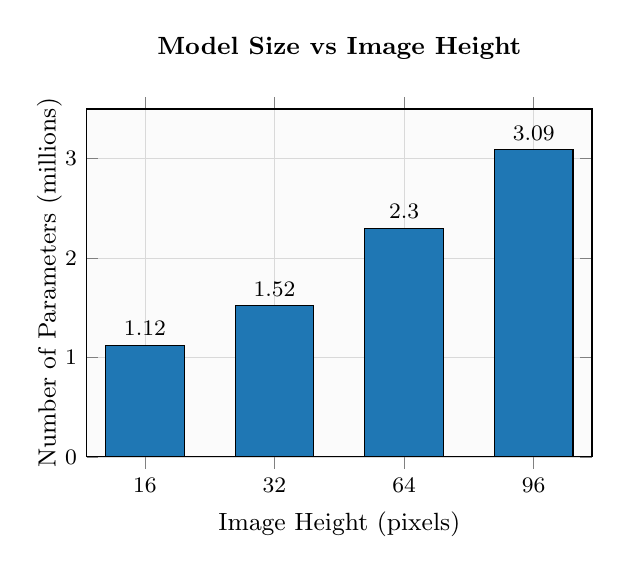
\begin{tikzpicture}
    \begin{axis}[
        width=8cm,
        height=6cm,
        ybar,
        bar width=1cm,
        xlabel={Image Height (pixels)},
        ylabel={Number of Parameters (millions)},
        ylabel style={yshift=-0.2cm},
        symbolic x coords={16,32,64,96},
        xtick=data,
        ymin=0,
        ymax=3.5,
        nodes near coords,
        nodes near coords align={vertical},
        every node near coord/.style={font=\footnotesize},
        grid=both,
        grid style={line width=.1pt, draw=gray!10},
        major grid style={line width=.2pt,draw=gray!30},
        title={Model Size vs Image Height},
        axis background/.style={fill=gray!3},
        title style={yshift=3mm, font=\small\bfseries},
        label style={font=\small},
        tick label style={font=\footnotesize},
        enlarge x limits=0.15
    ]
    
    % Data from your parameters count
    \addplot[fill=barblue] coordinates {
        (16, 1.12)
        (32, 1.52)
        (64, 2.30)
        (96, 3.09)
    };
    
    \end{axis}
\end{tikzpicture}

\end{document}